%% Jinja2 LaTeX template for the Evaluation section (moved under scripts/reports/article)
\section{Avaliação}

\subsection{Configuração da máquina e alocação de recursos}
Kernel: Linux Thingsboard 6.8.0-85-generic #85-Ubuntu SMP PREEMPT_DYNAMIC Thu Sep 18 15:26:59 UTC 2025 x86_64 x86_64 x86_64 GNU/Linux\\
CPU: Intel(R) Xeon(R) Silver 4310 CPU @ 2.10GHz
BIOS Model name:                      RHEL 7.6.0 PC (i440FX + PIIX, 1996)  CPU @ 2.0GHz (vCPU(s): 240)\\
Memória total: 15.67 GiB\\
Espaço em disco disponível no diretório do projeto: 172.07 GiB (rotacional: 1)\\

\subsection{Metodologia e definição de ODTE}
O experimento segue a metodologia descrita na Seção~\ref{sec:methodology}. A métrica ODTE (On-time Delivery Efficiency) é calculada por sensor sobre janelas de observação e reportada em porcentagem. Os detalhes de agregação usados nesta geração automática são: usamos médias ponderadas por número de mensagens quando disponíveis; também preservamos contagens de sensores ativos para referência.

\subsection{Resultados e discussão}
% Overview aggregated values (single/latest test used above)
\paragraph{Resumo agregado}
Sensores configurados (ODTE rows): 47\\
\vspace{1ex}

% Per-profile comparisons
\subsubsection{Comparação entre profiles}
Os testes foram agrupados por profile (ex.: \texttt{urllc}, \texttt{eMBB}, \texttt{best_effort}). Para cada profile selecionamos o "melhor" cenário usando a heurística: primeiro priorizamos ODTE média ponderada (A\%) mais alta; em caso de empate, priorizamos menor P95 S2M. A tabela a seguir resume o melhor cenário encontrado para cada profile.

\begin{tabular}{l l r r r r}
\textbf{Profile} & \textbf{Melhor teste} & \textbf{S2M msgs} & \textbf{S2M P95 (ms)} & \textbf{M2S P95 (ms)} & \textbf{ODTE A\%} \\
\hline

urllc & test_20251007T165815Z_urllc & 1809 & 173.8 & 605.3 & 63.60 \\

eMBB & test_20251007T171958Z_embb & 323 & 9479.2 & 1794.2 & 51.48 \\

best_effort & test_20251007T173922Z_best_effort & 87 & 8903.7 & 0.0 & 48.97 \\

\end{tabular}

\vspace{1ex}
\subsubsection{Discussão dos melhores cenários}

\paragraph{Profile: urllc}
O melhor teste identificado para o profile \texttt{ urllc } foi: \texttt{ test_20251007T165815Z_urllc }. Este cenário apresenta ODTE ponderada de 63.60\%, P95 S2M de 173.8 ms e P95 M2S de 605.3 ms. Comentários: 

\paragraph{Profile: eMBB}
O melhor teste identificado para o profile \texttt{ eMBB } foi: \texttt{ test_20251007T171958Z_embb }. Este cenário apresenta ODTE ponderada de 51.48\%, P95 S2M de 9479.2 ms e P95 M2S de 1794.2 ms. Comentários: 

\paragraph{Profile: best_effort}
O melhor teste identificado para o profile \texttt{ best_effort } foi: \texttt{ test_20251007T173922Z_best_effort }. Este cenário apresenta ODTE ponderada de 48.97\%, P95 S2M de 8903.7 ms e P95 M2S de 0.0 ms. Comentários: 


% Include plots and per-sensor tables for each selected best test
\section{Detalhes dos melhores cenários}

\subsection{Teste: test_20251007T165815Z_urllc (profile: urllc)}
\paragraph{Plots}


\begin{figure}[ht]
	\centering
	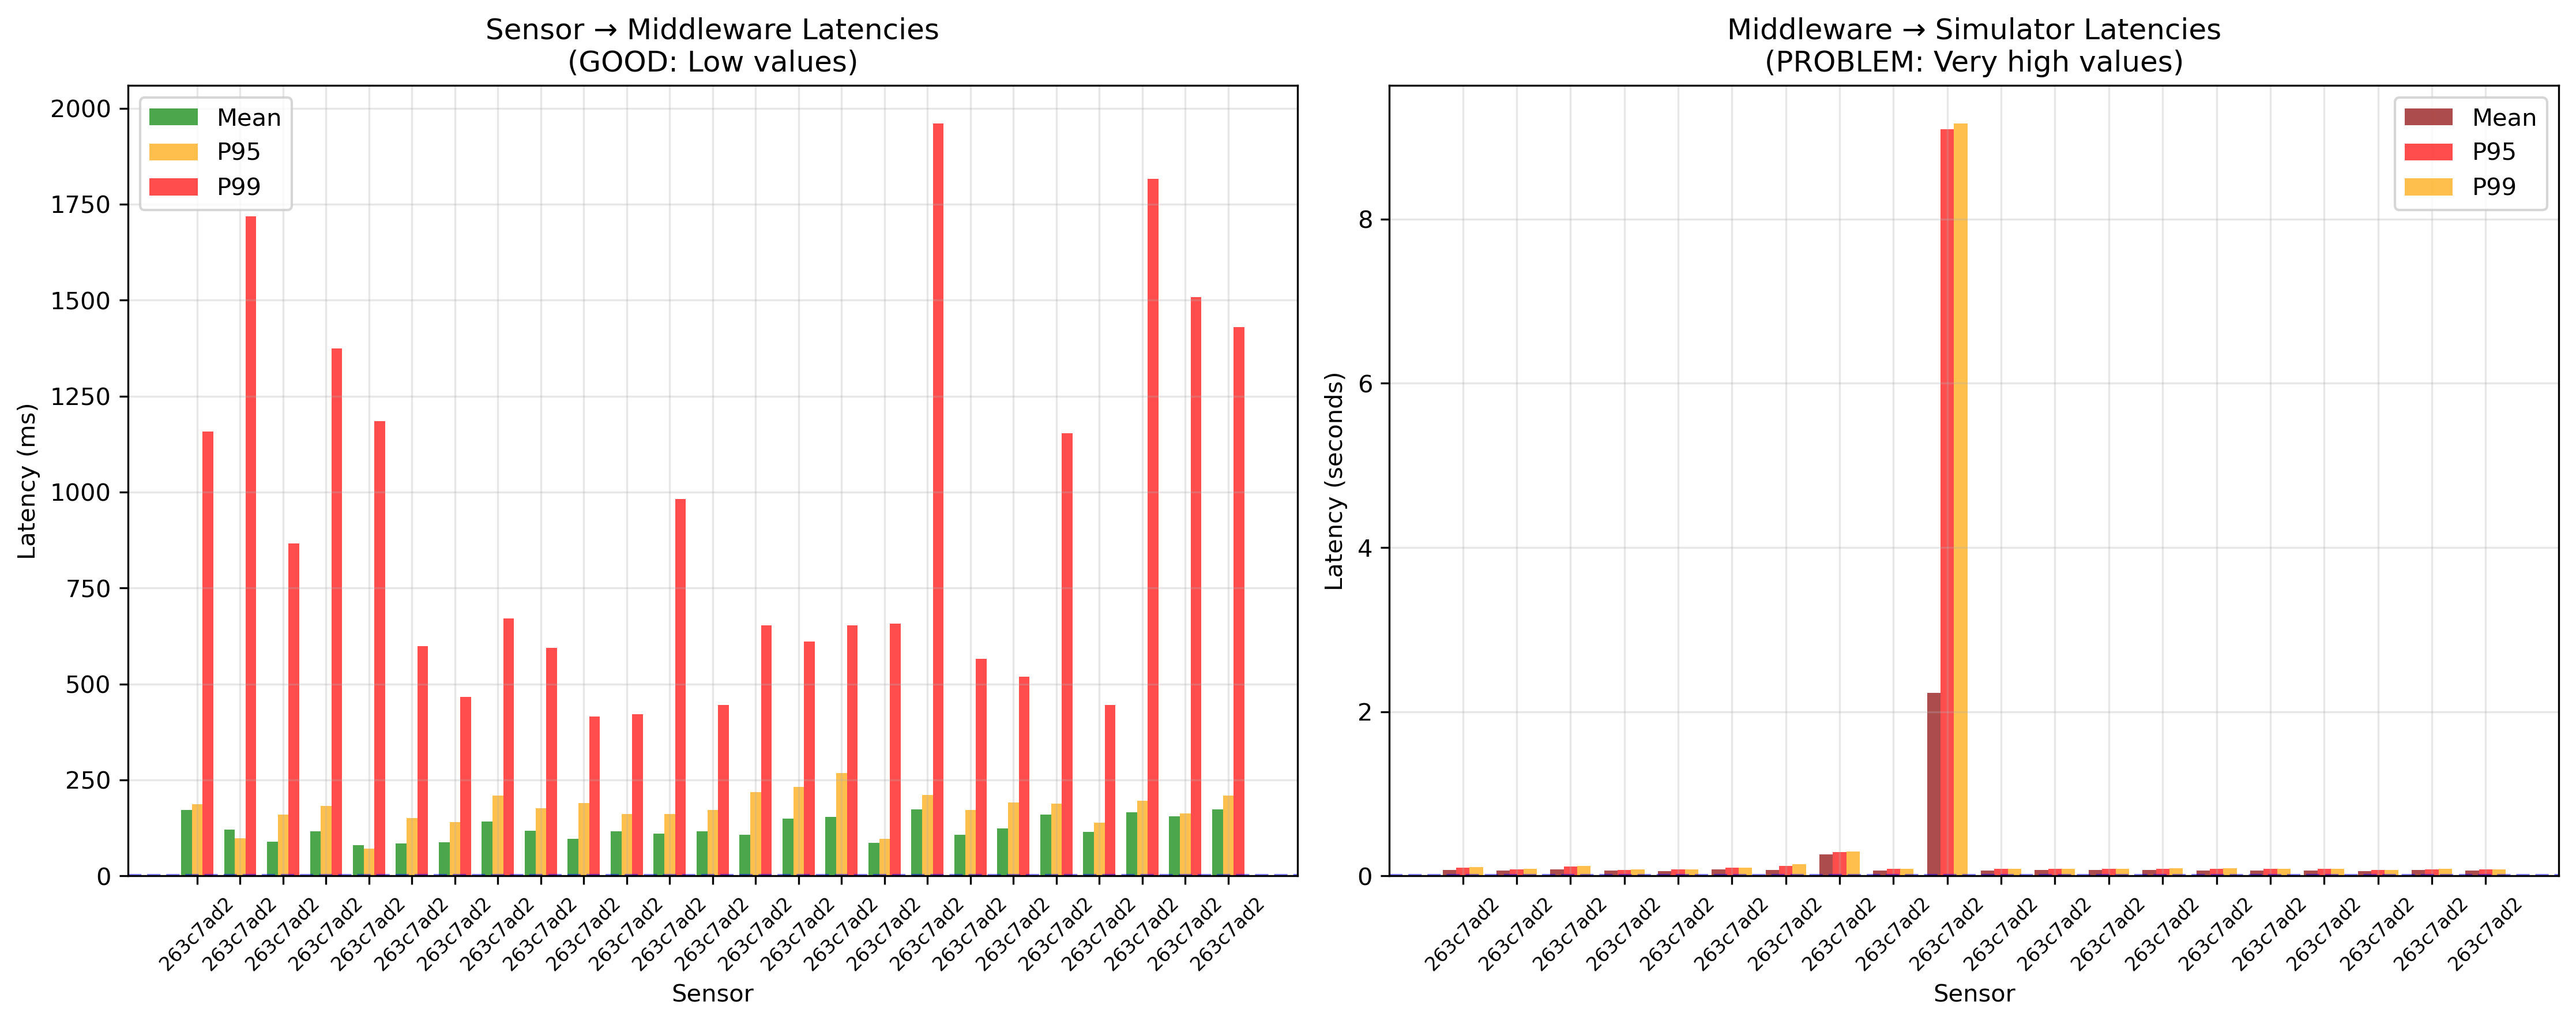
\includegraphics[width=0.8\linewidth]{ article/plots/urllc/urllc_latency_comparison.png }
	\caption{Plot gerado para test_20251007T165815Z_urllc: urllc_latency_comparison.png }
\end{figure}

\begin{figure}[ht]
	\centering
	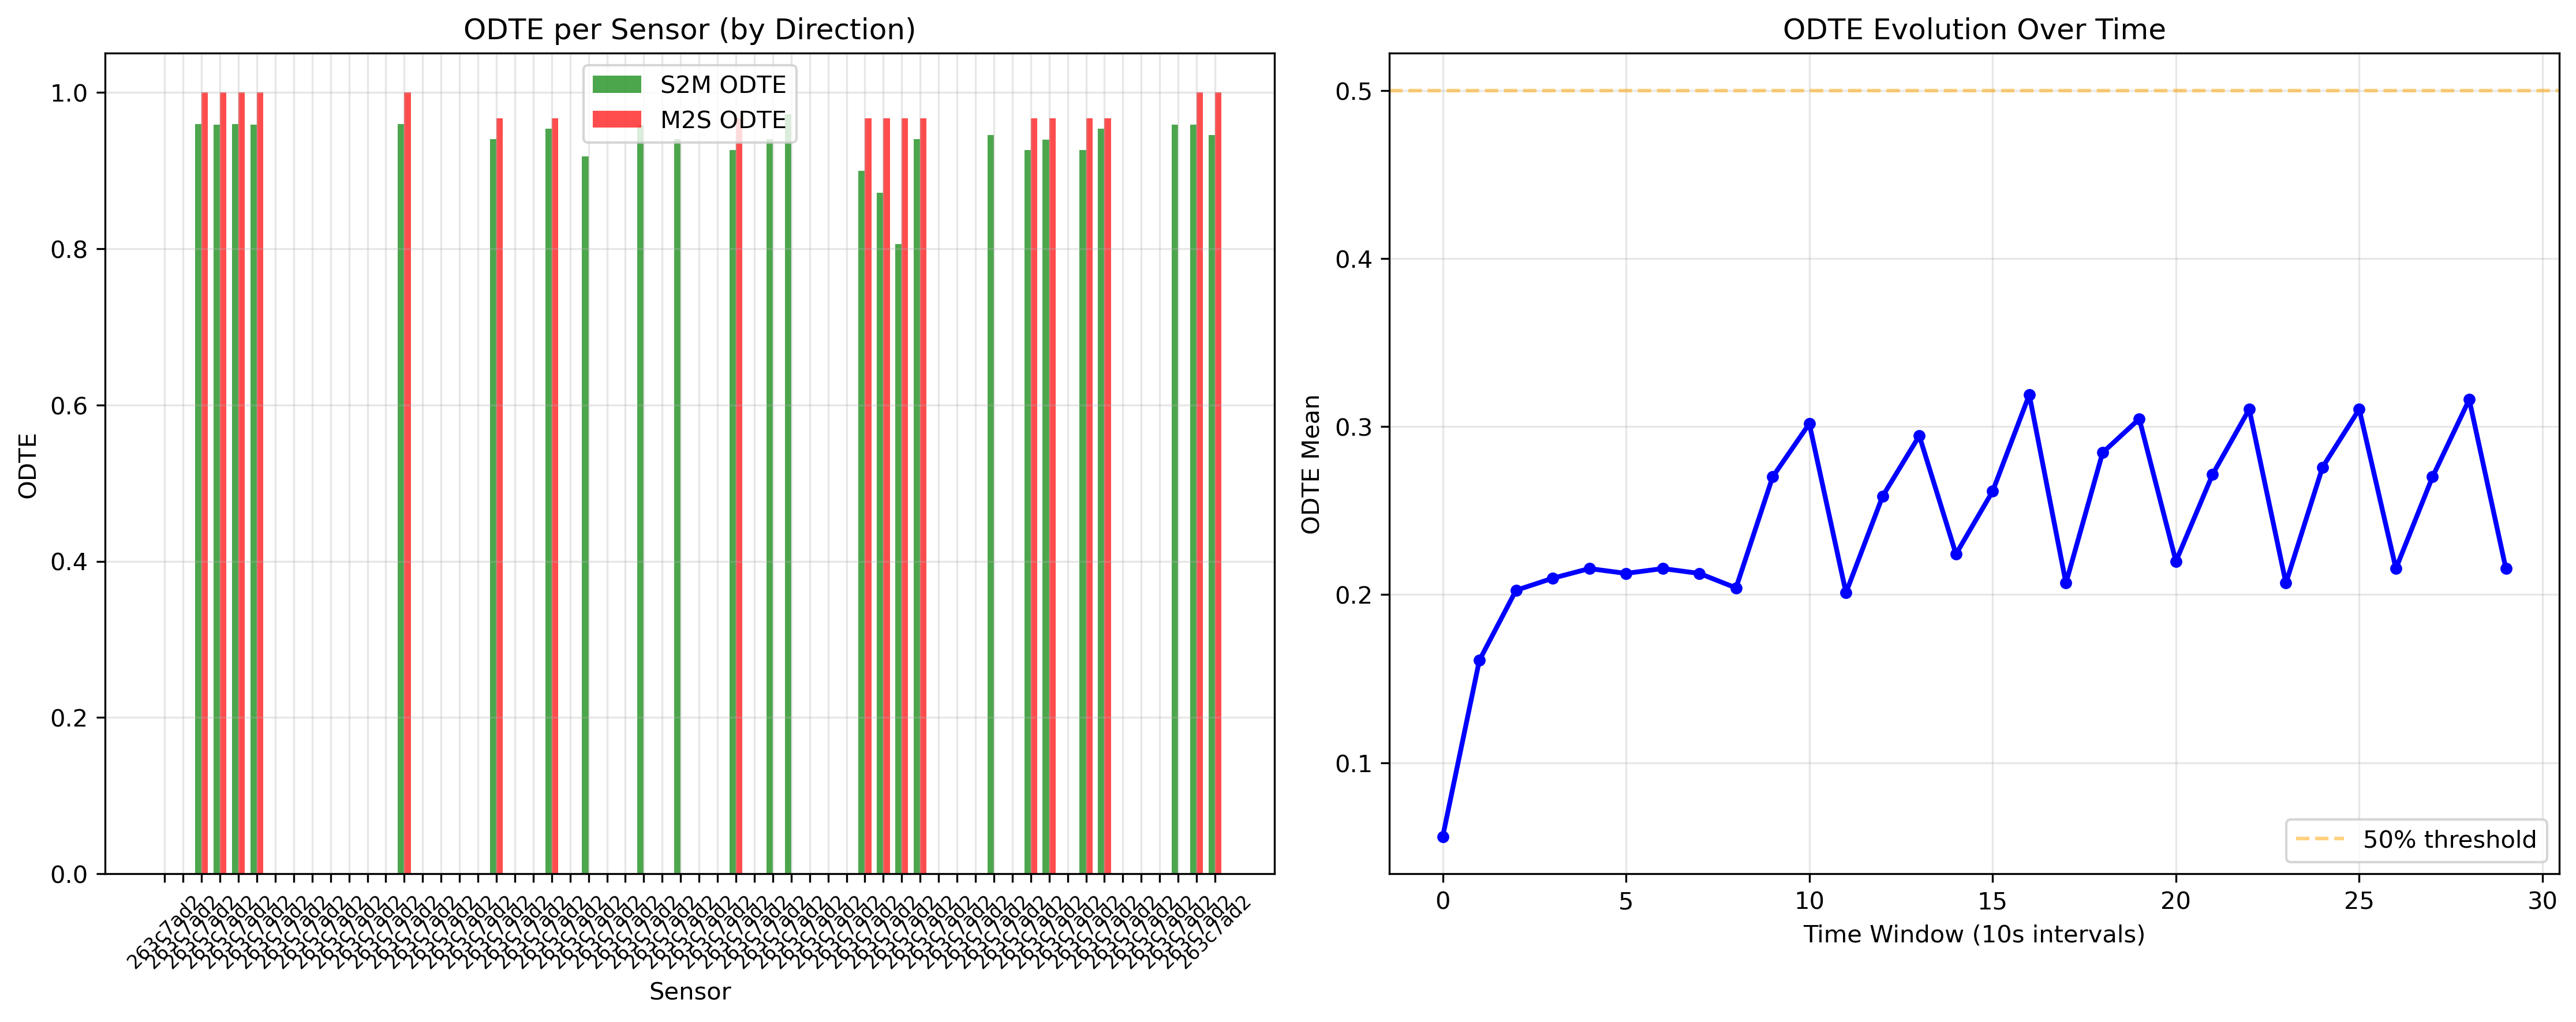
\includegraphics[width=0.8\linewidth]{ article/plots/urllc/urllc_odte_analysis.png }
	\caption{Plot gerado para test_20251007T165815Z_urllc: urllc_odte_analysis.png }
\end{figure}

\begin{figure}[ht]
	\centering
	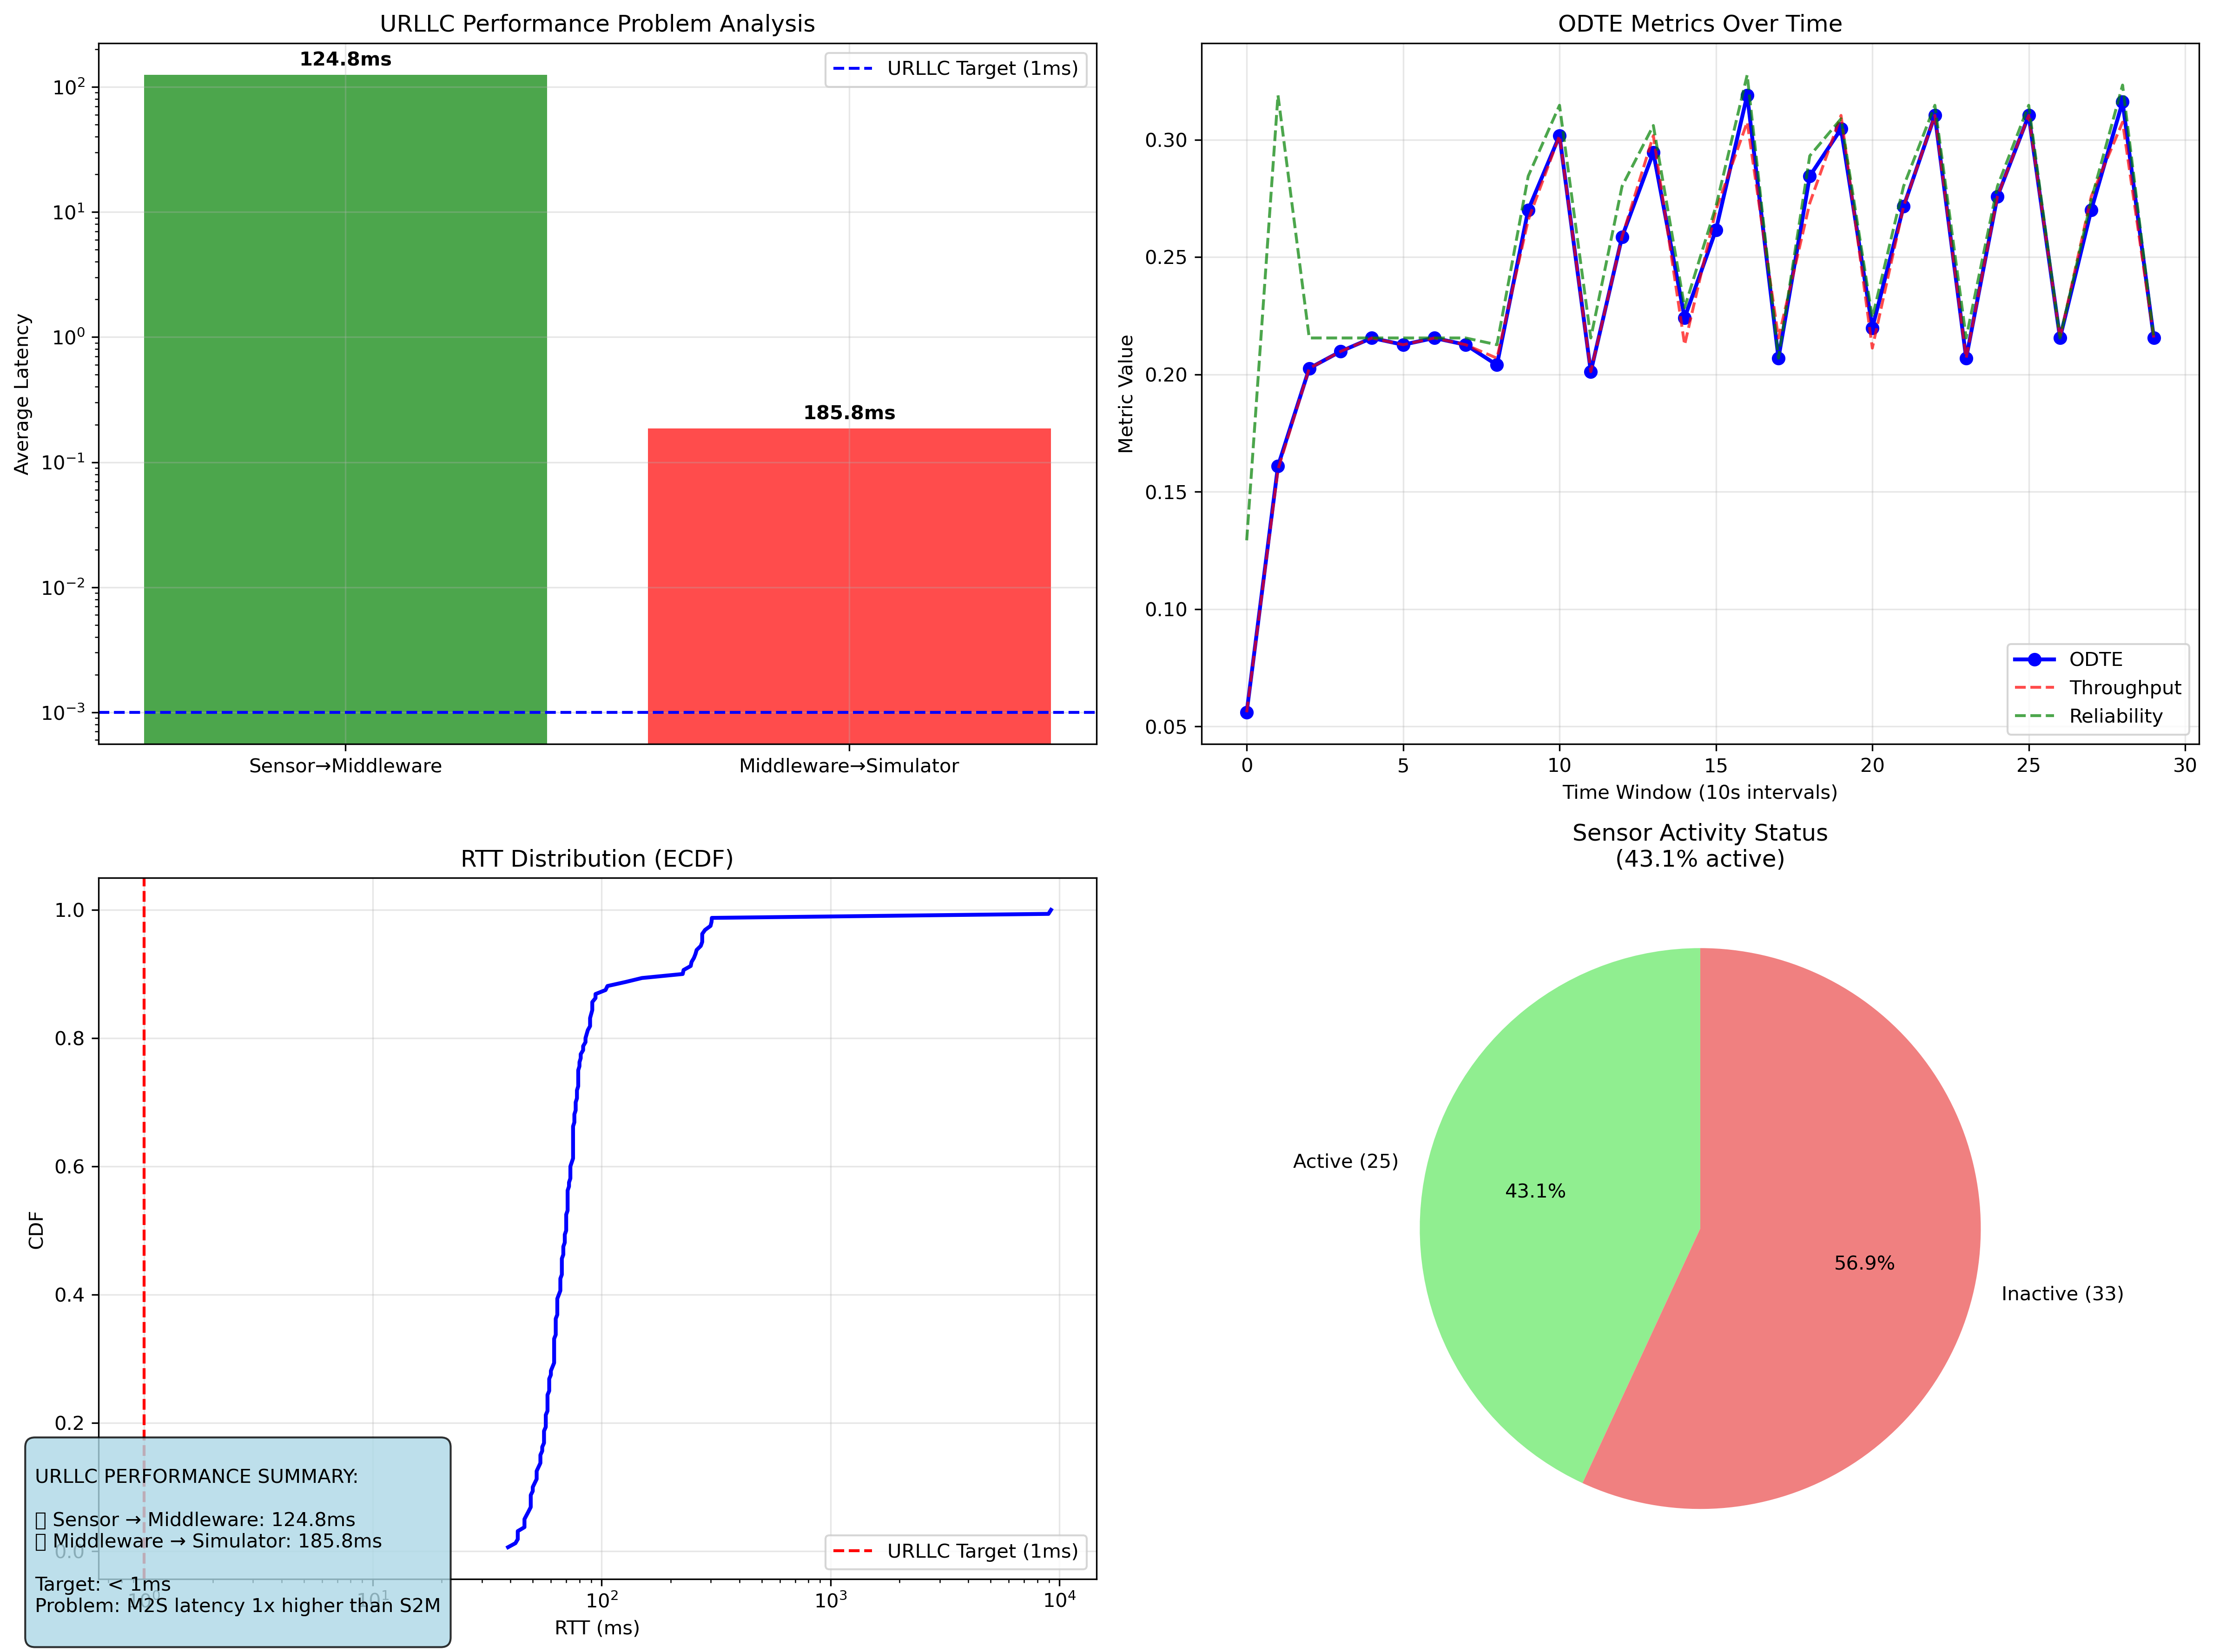
\includegraphics[width=0.8\linewidth]{ article/plots/urllc/urllc_problem_analysis.png }
	\caption{Plot gerado para test_20251007T165815Z_urllc: urllc_problem_analysis.png }
\end{figure}



\paragraph{Tabela por sensor}

\begin{longtable}{l r r r r}
	\textbf{Sensor} & \textbf{sim_sent} & \textbf{middts_sent} & \textbf{A\%} & \textbf{ODTE\_m2s\_capped} \\
\hline

1f3f0880-9ded-11f0-a687-8fcd263c7ad2 & 74 & 8 & 100.0 & 1.000 \\

1f3f0882-9ded-11f0-a687-8fcd263c7ad2 & 74 & 8 & 100.0 & 1.000 \\

20901990-9ded-11f0-a687-8fcd263c7ad2 & 74 & 7 & 100.0 & 1.000 \\

1f3f0881-9ded-11f0-a687-8fcd263c7ad2 & 73 & 8 & 100.0 & 1.000 \\

1f3f0883-9ded-11f0-a687-8fcd263c7ad2 & 73 & 8 & 100.0 & 1.000 \\

214279a0-9ded-11f0-a687-8fcd263c7ad2 & 73 & 8 & 100.0 & 0.000 \\

22e77710-9ded-11f0-a687-8fcd263c7ad2 & 73 & 8 & 100.0 & 0.000 \\

2459cbc0-9ded-11f0-a687-8fcd263c7ad2 & 73 & 8 & 100.0 & 0.000 \\

25a7cf90-9ded-11f0-a687-8fcd263c7ad2 & 73 & 8 & 100.0 & 1.000 \\

26c1f220-9ded-11f0-a687-8fcd263c7ad2 & 73 & 8 & 100.0 & 1.000 \\

2137f250-9ded-11f0-a687-8fcd263c7ad2 & 72 & 8 & 96.7 & 0.967 \\

213ef730-9ded-11f0-a687-8fcd263c7ad2 & 72 & 8 & 96.7 & 0.967 \\

21dfa400-9ded-11f0-a687-8fcd263c7ad2 & 72 & 16 & 96.7 & 0.000 \\

21f21a90-9ded-11f0-a687-8fcd263c7ad2 & 72 & 8 & 96.7 & 0.967 \\

21f798d0-9ded-11f0-a687-8fcd263c7ad2 & 72 & 0 & 96.7 & 0.000 \\

229697f0-9ded-11f0-a687-8fcd263c7ad2 & 72 & 8 & 96.7 & 0.967 \\

22a0d120-9ded-11f0-a687-8fcd263c7ad2 & 72 & 8 & 96.7 & 0.967 \\

22a56501-9ded-11f0-a687-8fcd263c7ad2 & 72 & 8 & 96.7 & 0.967 \\

233a7910-9ded-11f0-a687-8fcd263c7ad2 & 72 & 8 & 96.7 & 0.967 \\

2347bf80-9ded-11f0-a687-8fcd263c7ad2 & 72 & 8 & 96.7 & 0.967 \\

234bde30-9ded-11f0-a687-8fcd263c7ad2 & 72 & 8 & 96.7 & 0.967 \\

216a4cf0-9ded-11f0-a687-8fcd263c7ad2 & 71 & 8 & 100.0 & 0.000 \\

21ffaf20-9ded-11f0-a687-8fcd263c7ad2 & 71 & 16 & 100.0 & 0.000 \\

2296e610-9ded-11f0-a687-8fcd263c7ad2 & 71 & 8 & 96.7 & 0.967 \\

233c9bf0-9ded-11f0-a687-8fcd263c7ad2 & 71 & 8 & 96.7 & 0.967 \\

22899fa0-9ded-11f0-a687-8fcd263c7ad2 & 0 & 7 & 40.0 & 0.000 \\

2354b7d0-9ded-11f0-a687-8fcd263c7ad2 & 0 & 7 & 40.0 & 0.000 \\

213ed020-9ded-11f0-a687-8fcd263c7ad2 & 0 & 15 & 33.3 & 0.000 \\

215ae3a0-9ded-11f0-a687-8fcd263c7ad2 & 0 & 8 & 26.7 & 0.000 \\

21ec7540-9ded-11f0-a687-8fcd263c7ad2 & 0 & 14 & 26.7 & 0.000 \\

22293020-9ded-11f0-a687-8fcd263c7ad2 & 0 & 7 & 26.7 & 0.000 \\

22acb800-9ded-11f0-a687-8fcd263c7ad2 & 0 & 7 & 26.7 & 0.000 \\

1f3e6c40-9ded-11f0-a687-8fcd263c7ad2 & 0 & 7 & 23.3 & 0.000 \\

1f3e9350-9ded-11f0-a687-8fcd263c7ad2 & 0 & 7 & 23.3 & 0.000 \\

1f3f2f90-9ded-11f0-a687-8fcd263c7ad2 & 0 & 7 & 23.3 & 0.000 \\

1f3ff2e0-9ded-11f0-a687-8fcd263c7ad2 & 0 & 7 & 23.3 & 0.000 \\

1f4019f0-9ded-11f0-a687-8fcd263c7ad2 & 0 & 7 & 23.3 & 0.000 \\

214056c0-9ded-11f0-a687-8fcd263c7ad2 & 0 & 14 & 23.3 & 0.000 \\

2143b220-9ded-11f0-a687-8fcd263c7ad2 & 0 & 7 & 23.3 & 0.000 \\

21e04040-9ded-11f0-a687-8fcd263c7ad2 & 0 & 7 & 23.3 & 0.000 \\

21f771c0-9ded-11f0-a687-8fcd263c7ad2 & 0 & 14 & 23.3 & 0.000 \\

22890360-9ded-11f0-a687-8fcd263c7ad2 & 0 & 7 & 23.3 & 0.000 \\

22af5011-9ded-11f0-a687-8fcd263c7ad2 & 0 & 7 & 23.3 & 0.000 \\

22c65a80-9ded-11f0-a687-8fcd263c7ad2 & 0 & 7 & 23.3 & 0.000 \\

2335be20-9ded-11f0-a687-8fcd263c7ad2 & 0 & 7 & 23.3 & 0.000 \\

233e97c0-9ded-11f0-a687-8fcd263c7ad2 & 0 & 7 & 23.3 & 0.000 \\

23557b20-9ded-11f0-a687-8fcd263c7ad2 & 0 & 7 & 23.3 & 0.000 \\

236b2600-9ded-11f0-a687-8fcd263c7ad2 & 0 & 7 & 23.3 & 0.000 \\

\end{longtable}


